\begin{figure}[ht]
\centering
\caption*{Schéma de pré-tri}
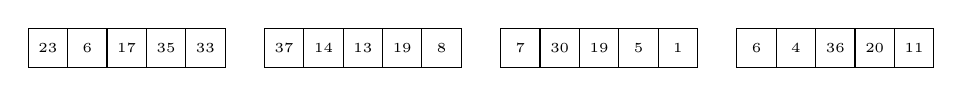
\begin{tikzpicture}[scale=0.5]
%%%%%%%%%%%%%%%%%%%%%%%%%%%%%%%%%%%%%%%%%%%%%%%%%%%%%%%%
% STYLE
\tikzstyle{case}=[rectangle,draw,minimum width=0.5cm,minimum height=0.5cm, font=\tiny]
\tikzstyle{op}=[circle,draw]
\tikzstyle{txt}=[]

\tikzset{link/.style={->,>=stealth'}}

%%%%%%%%%%%%%%%%%%%%%%%%%%%%%%%%%%%%%%%%%%%%%%%%%%%%%%%%
% NODES
\node[case] (T00) at (0, 0) {$23$};
\node[case] (T01) at (1, 0) {$6$};
\node[case] (T02) at (2, 0) {$17$};
\node[case] (T03) at (3, 0) {$35$};
\node[case] (T04) at (4, 0) {$33$};

\node[case] (T06) at (6, 0) {$37$};
\node[case] (T07) at (7, 0) {$14$};
\node[case] (T08) at (8, 0) {$13$};
\node[case] (T09) at (9, 0) {$19$};
\node[case] (T10) at (10, 0) {$8$};

\node[case] (T12) at (12, 0) {$7$};
\node[case] (T13) at (13, 0) {$30$};
\node[case] (T14) at (14, 0) {$19$};
\node[case] (T15) at (15, 0) {$5$};
\node[case] (T16) at (16, 0) {$1$};

\node[case] (T18) at (18, 0) {$6$};
\node[case] (T19) at (19, 0) {$4$};
\node[case] (T20) at (20, 0) {$36$};
\node[case] (T21) at (21, 0) {$20$};
\node[case] (T22) at (22, 0) {$11$};


%%%%%%%%%%%%%%%%%%%%%%%%%%%%%%%%%%%%%%%%%%%%%%%%%%%%%%%%
% LINKS

\end{tikzpicture}
\end{figure}